\section{Тензоры}

В этом разделе будут введены некоторые операции над тензорами и изучено то, как они влияют на ранг.

Далее $\langle k,m,n \rangle:K^{k \times m} \times K^{m \times n} \to K^{k \times n}$ обозначает билинейное отображение, которое переводит $k \times m$-матрицу $A$ и $m \times n$-матрицу $B$ в их произведение $AB$. Потому как нет опасности запутаться, также будет обозначаться соответствующий тензор и множество билинейных форм
\[
	\left\{ \sum\limits_{\mu=1}^{m} X_{\kappa \mu} Y_{\mu \nu}| 1 \leq \kappa \leq k,\; 1 \leq \nu \leq n \right\}.
\]

\subsection{Перестановки}

Пусть $t \in K^{k \times m \times n}$ и $t = \sum_{j=1}^{r} t_j$ с триадами $t_j = a_{j1} \otimes a_{j2} \otimes a_{j3}, \; 1 \leq j \leq r $. Пусть $\pi \in S_3$. Для триады $t_j$ пусть $\pi t_j = a_{j \pi^{-1}(1)} \otimes a_{j \pi^{-1}(2)} \otimes a_{j \pi^{-1}(3)}$ и $\pi t = \sum_{j=1}^{r} \pi t_j$. Заданное таким образом отображение $\pi$ будет вполне определено, то есть не будет зависеть от способа декомпозиции $t$ в сумму триад. Чтобы это увидеть, пусть $t = \sum_{i=1}^{s} b_{i1} \otimes b_{i2} \otimes b_{i3}$ --- вторая декомпозиция $t$. Знаем, что
\[
	\sum_{j=1}^{r} a_{j1} \otimes a_{j2} \otimes a_{j3} = \sum_{i=1}^{s} b_{i1} \otimes b_{i2} \otimes b_{i3}.
\]
И хотим доказать, что
\[
	\sum_{j=1}^{r} a_{j \pi^{-1}(1)} \otimes a_{j \pi^{-1}(2)} \otimes a_{j \pi^{-1}(3)} = \sum_{i=1}^{s} b_{i \pi^{-1}(1)} \otimes b_{i \pi^{-1}(2)} \otimes b_{i \pi^{-1}(3)}.
\]
Пусть $a_{j1} = \left( a_{j11}, \dotsc, a_{j1k} \right)$ и $b_{i1} = \left( b_{i11}, \dotsc, b_{i1k} \right)$, и пусть $a_{j2}, \; a_{j3}, \; b_{j2}, \; b_{j3}$ задаются аналогично.
Получится, что у тензора $t$ в позиции $\left( e_1,e_2,e_3 \right)$ стоит
\[
	t_{e_1e_2e_3} = \sum\limits_{j=1}^{r} a_{j1e_1} \otimes a_{j2e_2} \otimes a_{j3e_3} = \sum\limits_{i=1}^{s} b_{i1e_1} \otimes b_{i2e_2} \otimes b_{i3e_3}.
\]
Таким образом, у тензора $\pi t$ в позиции $(e_1, e_2, e_3)$ стоит
\[
	\begin{array}{rcl}
	  \pi t_{e_1e_2e_3} & = & \sum\limits_{j=1}^{r} a_{j \pi^{-1}(1) e_{\pi^{-1}(1)}} \otimes a_{j \pi^{-1}(2) e_{\pi^{-1}(2)}} \otimes a_{j \pi^{-1}(3) e_{\pi^{-1}(3)}}\\
	  & = & \sum\limits_{i=1}^{s} b_{i \pi^{-1}(1) e_{\pi^{-1}(1)}} \otimes b_{i \pi^{-1}(2) e_{\pi^{-1}(2)}} \otimes b_{i \pi^{-1}(3) e_{\pi^{-1}(3)}}.
	\end{array}
\]
\begin{question}
  Не совсем понятно, как приведённое равенство доказывает утверждение о том, что действие вполне определено. 
\end{question}

\begin{figure}[H]
	\centering
    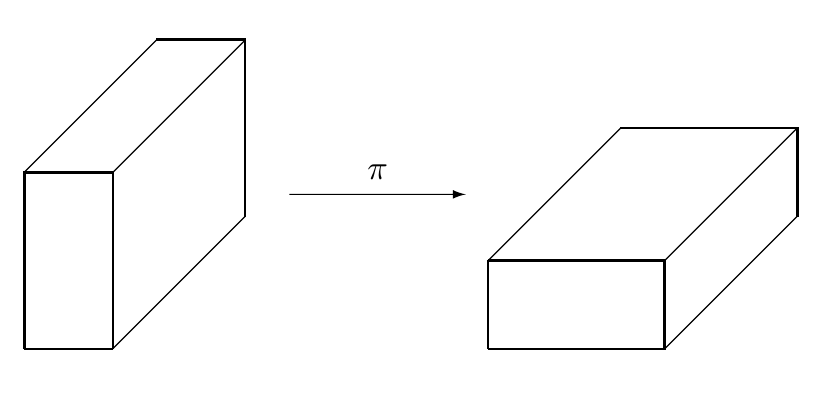
\includegraphics[width=0.5\textwidth]{figures/dimensions_permutation}
	\caption{Перестановка измерений}
	\label{fig:dimensions_permutation}
\end{figure}

Доказательство следующей леммы очевидно.
\begin{lemma}\label{lem:bi:4.3}
  $R(t) = R(\pi t)$
\end{lemma}

Кроме перестановки измерений тензора можно также переставлять его слои. Пусть $t=(t_{ij \ell}) \in K^{k \times m \times n}$ и $\sigma \in S_k$. Тогда для $t'=(t_{\sigma(i)j \ell})$, $R(t')=R(t)$.
\begin{figure}[H]
	\centering
    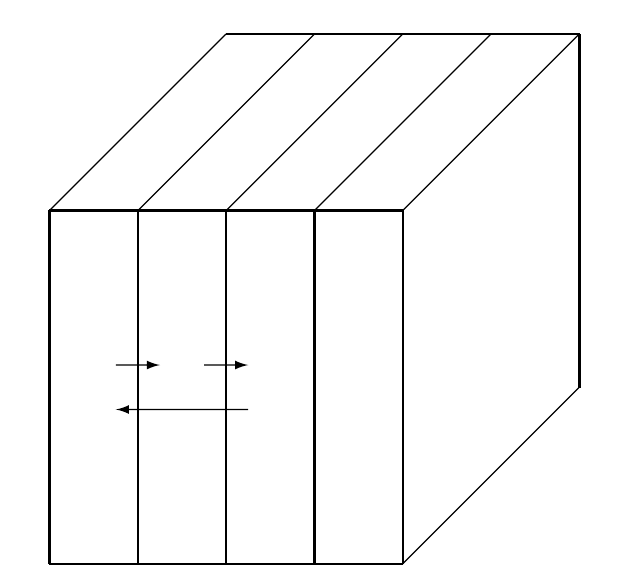
\includegraphics[width=0.5\textwidth]{figures/slices_permutation}
	\caption{Перестановка слоёв тензора}
	\label{fig:slices_permutation}
\end{figure}

В более общем смысле, пусть $A: K^{k} \to K^{k'}, B: K^{m} \to K^{m'}$ и $C: K^{n} \to K^{n'}$ являются гомоморфизмами. Пусть $t = \sum_{j=1}^{r} t_j$ с триадами $t_j = a_{j1} \otimes a_{j2} \otimes a_{j3}$. Для триад $t_j$ зададим
\[
	(A \otimes B \otimes C) t_j = A(a_{j1}) \otimes B(a_{j2}) \otimes C(a_{j3})
\]
и
\[
	(A \otimes B \otimes C) t = \sum_{j=1}^r (A \otimes B \otimes C) t_j.
\]
Также как и выше, если рассмотреть отдельный элемент $t$, то легко увидеть, что это отображение вполне определено.

Доказательство следующей леммы очевидно.
\begin{lemma}\label{lem:bi:4.4}
  $R((A \otimes B \otimes C)t) \leq R(t)$.
\end{lemma}
Равенство выполняется, если $A, B$ и $C$ изоморфизмы.

Как же выглядит тензор матричного умножения? Вспомним, что его билинейные формы задаются как
\[\label{matrix_tensor}
	Z_{\kappa \nu} = \sum\limits_{\mu=1}^{m} X_{\kappa \mu} Y_{\mu \nu}, \; 1 \leq \kappa \leq k,\; 1 \leq \nu \leq n.
\]
Элементы соответствующего тензора
\[
	\left( t_{\kappa \bar{\mu}, \mu \bar{\nu}, \nu \bar{\kappa}} \right) = t \in K^{(k \times m) \times (m \times n) \times (n \times k)}
\]
задаются как
\[
	t_{\kappa \bar{\mu}, \mu \bar{\nu}, \nu \bar{\kappa}} = \delta_{\bar{\kappa}\kappa} \delta_{\bar{\mu} \mu} \delta_{\bar{\nu} \nu},
\]
где $\delta_{ij}$ --- это дельта Кронекера --- функция равная 1, если $i=j$, и 0, если $i \neq j$. (Здесь каждое измерение тензора индексируется двумя числами, что является отражением способа нумерации элементов в матрице. Если вам так больше нравится, то можно нумеровать элементы тензора индексами $1, \dotsc, km; 1, \dotsc mn; 1, \dotsc nk$. Также были <<транспонированы>> индексы в третьем слое, чтобы тензор имел более симметричный вид.) 

Пусть $\pi = \left( 1\;2\;3 \right)$. Тогда для $t' := \pi t \in K^{(n \times k) \times (k \times m) \times (m \times n)}$ получим
\[
	\begin{array}{lcl}
		t'_{\nu \bar{\kappa}, \kappa \bar{\mu}, \mu \bar{\nu}  } & = & \delta_{\bar{\nu} \nu} \delta_{\bar{\kappa}\kappa} \delta_{\bar{\mu} \mu} \\
		& = & \delta_{\bar{\kappa}\kappa} \delta_{\bar{\mu} \mu} \delta_{\bar{\nu} \nu}\\
		& = & t_{\kappa \bar{\mu}, \mu \bar{\nu}, \nu \bar{\kappa}   }.
	\end{array}
\]
Поэтому $t' = \left\langle n,k,m \right\rangle$ (напомню, что $t = \left\langle k,m,n \right\rangle$). Ничто не мешает применить $\pi$ к $t'$, и тогда $\pi t' = \left\langle m,n,k \right\rangle$. Отсюда по лемме \ref{lem:bi:4.3} $R \left( \left\langle k, m, n \right\rangle \right) = R \left( \left\langle n, k, m \right\rangle \right) = R \left( \left\langle m, n, k \right\rangle \right)$.

Теперь пусть $t'':=\left( t_{\mu \bar{\kappa}, \nu \bar{\mu}, \kappa \bar{\nu} } \right) \in K^{(m \times k) \times (n \times m) \times (k \times n)}$. Получим, что $R(t)=R(t'')$, потому как перестановка <<внутренних>> индексов соответствует перестановке слоёв тензора.

Затем положим $\pi = (1\;2)(3)$. И пусть $t''':= \pi t'' \in K^{(n \times m) \times (m \times k) \times (k \times n)}$. Получим, что
\begin{align*}
     t'''_{\nu \bar{\mu}, \mu \bar{\kappa}, \kappa \bar{\nu}   } & = \delta_{\mu \bar{\mu} } \delta_{\kappa \bar{\kappa} } \delta_{\nu \bar{\nu} }\\
     & = t_{\bar{\kappa}\mu, \bar{\mu} \nu, \bar{\nu} \kappa}.
\end{align*}
Отсюда $R \left( \left\langle k,m,n \right\rangle \right) = R \left( \left\langle n,m,k \right\rangle \right)$. Это соответствует известному факту для матриц:
\[
	\underset{k \times m}{A} \cdot \underset{m \times n}{B} = \underset{k \times n}{C} \implies \underset{n \times m}{B^T} \cdot \underset{m \times k}{A^T} = \underset{n \times k}{C^T}.
\]

\subsection{Произведение и сумма}

Пусть $t \in K^{k \times m \times n}$ и $t' \in K^{k' \times m' \times n'}$. \textbf{Прямой суммой} $t$ и $t'$ называют тензор $s := t \oplus t' \in K^{(k+k') \times (m+m') \times (n+n')}$, задаваемый как:
\[
	s_{\kappa \mu \nu} = 
	\begin{cases}
	  t_{\kappa \mu \nu} & \text{если } 1 \leq \kappa \leq k, 1 \leq \mu \leq m, 1 \leq \nu \leq n\\
	  t'_{\kappa - k, \mu - m, \nu -n} & \parbox[t]{.6\textwidth}{если  ${k+1 \leq \kappa \leq k+k'}, {m+1 \leq \mu \leq m+m'}, {n+1 \leq \nu \leq n+n'}$} \\
	  0 & \text{иначе }
	\end{cases}
\]
\begin{figure}[H]
	\centering
    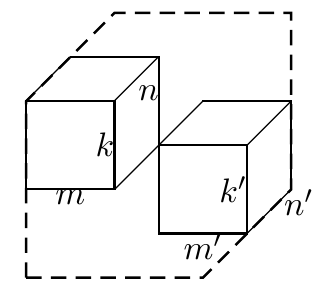
\includegraphics[width=0.25\textwidth]{figures/direct_sum}
	\caption{Прямая сумма двух тензоров}
	\label{fig:direct_sum}
\end{figure}

\begin{lemma}\label{lem:bi:4.5}
  $R \left( t \oplus t' \right) \leq R(t) + R(t')$. 
\end{lemma}
\begin{proof}
  Пусть $t = \sum_{i=1}^r u_i \otimes v_i \otimes w_i$ и $t' = \sum_{i=1}^{r'} u_i' \otimes v_i' \otimes w_i'$. Пусть
  \begin{align*}
    \widehat{u}_i & = (\underbrace{u_{i1}, \dotsc, u_{ik}}_{u_i},\underbrace{0, \dotsc, 0}_{k'})   \text{ и }\\
    \widehat{u}_i' & = (\underbrace{0, \dotsc, 0}_{k}, \underbrace{u_{i1}', \dotsc, u_{ik}'}_{u_i'}).
  \end{align*}
  и определим $\widehat{v}_i, \widehat{w}_i$ и $\widehat{v}_i', \widehat{w}_i'$ аналогично. Простые вычисления показывают, что
  \[
  	t \oplus t' = \sum_{i=1}^{r} \widehat{u}_i \otimes \widehat{v}_i \otimes \widehat{w}_i + \sum_{j=1}^{r'} \widehat{u}_j' \otimes \widehat{v}_j' \otimes \widehat{w}_j',
  \]
  то есть $R(t \oplus t') \leq r + r' = R(t) + R(t')$.
\end{proof}

\begin{reseach}[Аддитивная гипотеза Штрассена]\label{res:bi:4.1}
	Показать, что для всех тензоров $t$ и $t'$: $R(t \oplus t') = R(t) + R(t')$, то есть в лемме выше всегда имеет место равенство.
\end{reseach}

\textbf{Тензорное произведение} $t \otimes t' \in K^{kk' \times mm' \times nn'}$ двух тензоров $t \in K^{k \times m \times n}$ и $t' \in K^{k' \times m' \times n'}$ задаётся как 
\[
	t \otimes t' = \left( t_{\kappa \mu \nu} t'_{\kappa' \mu' \nu'} \right)_{\substack{
		1 \leq \kappa \leq k, \; 1 \leq \kappa' \leq k' \\
		1 \leq \mu \leq m, \; 1 \leq \mu' \leq m'\\
		1 \leq \nu \leq n, \; 1 \leq \nu' \leq n'}}
\]
\begin{figure}[H]
	\centering
    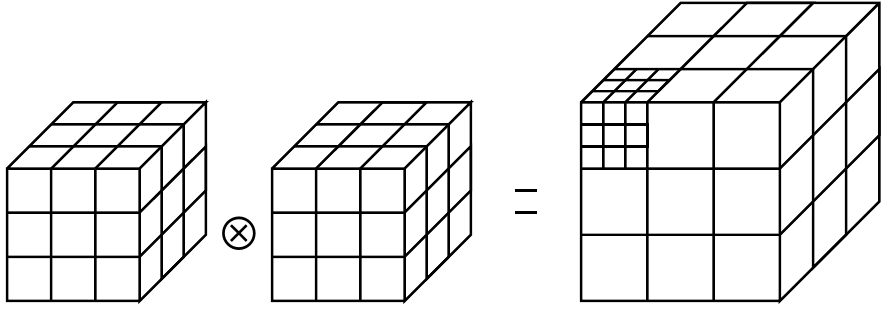
\includegraphics[width=0.75\textwidth]{figures/tensor_product}
	\caption{Тензорное произведение}
	\label{fig:tensor_product}
\end{figure}
\begin{lemma}
  $R \left( t \otimes t' \right) \leq R(t) R(t')$. 
\end{lemma}
\begin{proof}
  Пусть $t = \sum_{i=1}^r u_i \otimes v_i \otimes w_i$ и $t' = \sum_{i=1}^{r'} u_i' \otimes v_i' \otimes w_i'$. Пусть $u_i \otimes u_j' \overset{Def}{=} (u_{i \kappa} u_{j \kappa'}') \in K^{k k'}$
  Тем же образом определим $v_i \otimes v_j', w_i \otimes w_j'$. Имеем
  \begin{align*}
    (u_i \otimes u_j') \otimes (v_i \otimes v_j') \otimes (w_i \otimes w_j') & = (u_{i \kappa} u_{j \kappa'}' \cdot v_{j \mu} v_{j \mu'}' \cdot w_{i \nu} w_{j \nu'}')_{\substack{
		1 \leq \kappa \leq k, \; 1 \leq \kappa' \leq k' \\
		1 \leq \mu \leq m, \; 1 \leq \mu' \leq m'\\
		1 \leq \nu \leq n, \; 1 \leq \nu' \leq n'}} \\
		& \in K^{k k' \times m m' \times n n'} \cong K^{(k \times k') \times (m \times m') \times (n \times n')}   
  \end{align*}
  и
  \begin{align*}
    \sum_{i=1}^r \sum_{j=1}^{r'} (u_i \otimes u_j') \otimes (v_i \otimes v_j') \otimes (w_i \otimes w_j') & = 
    			\left( \sum_{i=1}^r \sum_{j=1}^{r'} u_{i \kappa} u_{j \kappa'}' v_{i \mu} v_{j \mu'}' w_{i \nu} w_{j \nu'}' \right)_{\substack{
		1 \leq \kappa \leq k, \; 1 \leq \kappa' \leq k' \\
		1 \leq \mu \leq m, \; 1 \leq \mu' \leq m'\\
		1 \leq \nu \leq n, \; 1 \leq \nu' \leq n'}}    \\
		& = \bigg( \underbrace{\left( \sum_{i=1}^r u_{i \kappa} v_{i \mu} w_{i \nu} \right)}_{t_{\kappa \mu \nu}} \cdot \underbrace{\left( \sum_{j=1}^{r'} u_{j \kappa'}' v_{j \mu'}' w_{j \nu'}' \right)}_{t_{\kappa' \mu' \nu'}'} \bigg)_{\substack{
		1 \leq \kappa \leq k, \; 1 \leq \kappa' \leq k' \\
		1 \leq \mu \leq m, \; 1 \leq \mu' \leq m'\\
		1 \leq \nu \leq n, \; 1 \leq \nu' \leq n'}}    \\
		& = t \otimes t',
  \end{align*}
  то есть $R(t \otimes  t') \leq r r' = R(t) R(t')$.
\end{proof}

Для тензорного произведения матричных умножений получим, что
\[
	\begin{array}{lcl}
		\left\langle k,m,n \right\rangle \otimes \left\langle k', m', n' \right\rangle	& = & \left( 
			\delta_{\kappa \bar{\kappa}} \delta_{\mu \bar{\mu}} \delta_{\nu \bar{\nu}} 
			\delta_{\kappa' \bar{\kappa'}} \delta_{\mu' \bar{\mu'}} \delta_{\nu' \bar{\nu'}}
		\right)\\
		& = & \left( \delta_{\kappa \bar{\kappa}} \delta_{\kappa' \bar{\kappa'}} \delta_{\mu \bar{\mu}} \delta_{\mu' \bar{\mu'}} \delta_{\nu \bar{\nu}} \delta_{\nu' \bar{\nu'}}\right)\\
		& = & \left( \delta_{(\kappa, \kappa'), (\bar{\kappa}, \bar{\kappa'})}, \delta_{(\mu, \mu'), (\bar{\mu}, \bar{\mu'})}, \delta_{(\nu, \nu'), (\bar{\nu}, \bar{\nu'})} \right)\\
		& = & \left\langle kk', mm', nn' \right\rangle
	\end{array}
\]

Таким образом, тензорное произведение двух матричных тензоров будет снова матричным тензором, но больших размеров, что соответствует тождеству для произведений Кронекера
\[
	(A \otimes B)(A' \otimes B') = (AA' \otimes BB').
\]

\begin{theorem}\label{th:4.7}
	Для всех $k,m,n$ получим, что $(kmn)^{\omega/3} \leq R(\left\langle k,m,n \right\rangle)$.
\end{theorem}
\begin{proof}
	Пусть $R(\left\langle k,m,n \right\rangle) \leq r$, тогда $R(\left\langle n,k,m \right\rangle) \leq r$ и $R(\left\langle m,n,k \right\rangle) \leq r$. Поэтому
	\[
		R(\underbrace{\left\langle k,m,n \right\rangle \otimes \left\langle n,k,m \right\rangle \otimes \left\langle m,n,k \right\rangle}_{=\left\langle kmn, kmn, kmn \right\rangle}) \leq r^3.
	\]
	Положив, $M=kmn$ получим $R(\langle M , M, M \rangle) \leq r^3$. Тогда для всех $N \geq 1$, при помощи дополнения до
следующей наибольшей степени $M^i$ числа $M$,
	\[
		R(\left\langle N,N,N \right\rangle) \leq R(\left\langle M^i, M^i, M^i \right\rangle) \leq r^{3i} = (M^{3 \log_M r})^i = (M^i)^{3 \log_M r} = O(N^{3 \log_M r})
	\]
	 Поэтому 
	  \begin{align*}
	    \omega & \leq 3 \log_M r   \\
	    M^{\omega/3} & \leq r \\
	    (k m n)^{\omega/3} & \leq r.
	  \end{align*} 
	По определению $R(\left\langle k,m,n \right\rangle)$ является положительным целым, и так как $R(\left\langle k,m,n \right\rangle) \leq R(\left\langle k,m,n \right\rangle)$ то получим, что $(k m n)^{\omega/3} \leq R(\left\langle k,m,n \right\rangle)$. Это будет эквивалентно $\omega \leq \frac{\log R(\left\langle k,m,n \right\rangle)}{\log (kmn)^{1/3}}$.
\end{proof}

Стандартное применение теоремы \ref{th:4.7} будет следующим: допустим, что доказано $R(\left\langle 2,2,2 \right\rangle) \leq 7$ (в данном случае это результат Штрассена 1969 года \cite{Strassen:1969}), отсюда будет следовать нетривиальная верхняя оценка на экспоненту матричного умножения 
\[
	\omega \leq 3 \log_{2^3} 7 = \log_2 7 \approx 2.81.
\]










